\section{Introduction}

Large datacenters have been at the heart of the increasingly content-centric internet for the past decade. Many architectures have been proposed, such as fat-tree, BCube (Guo et al 2009), and Jellyfish (Singla et al 2012), a choice which does not come without tradeoffs. On the one hand, fat-trees are deterministic, symmetric architectures with constant inter-server path lengths and minimal room for implementation errors. Symmetric architectures work well for pre-planned, fixed-size data centers when the equipment is homogeneous and known in advance. However, these assumptions break down once we consider incremental expansion and flexibility of design as requirements.

Jellyfish attempts to mitigate this problem by following a quasi-random iterative approach to incrementally add equipment to the network, thus lending itself for expansion in variable-length increments. Nevertheless, after building the initial network, and given that edges are not removed once added (with a very specific exception), it’s still unclear whether the process of incrementally expanding Jellyfish maintains the desired properties of random graphs at scale, such as short paths, or too heavily depends on the existing network. Moreover, Jellyfish doesn’t address the problem of homogeneous equipment: all switches are assumed to have the same number of ports, and servers only have 1 port, i.e. sit at the edge of the network.

In this paper, we reproduce the main findings of \textit{Scafida: A Scale-Free Network Inspired Data Center Architecture}. The paper proposes and evaluates Scafida, a datacenter topology that breaks the symmetry traditionally found in state-of-the-art architectures, while allowing for arbitrary numbers of heterogenous equipment in the network and involving servers with more than one port in the routing process. The Scafida topology is inspired by scale-free networks (e.g. ordinary Barabasi-Albert topology), and attempts to exploit all the desirable properties that come along, namely short paths and high fault tolerance (path redundancy.) However, it imposes the additional constraint of limiting the degrees of nodes in the network, since neither switches nor servers can have arbitrary numbers of ports in practice. The original paper finds that such degree constraints have little negative effect on the resulting topology, and that Scafida has favorable properties, such as low mean path lengths, high throughput, and fault tolerance in the face of significant failures, all of which are comparable to state-of-the-art topologies, despite its asymmetric structure.

Our reproduction starts with understanding the ordinary Barabasi-Albert scale-free network, and implementing the Scafida variation to limit node degrees and parametrize for heterogeneous equipment; as in the Scafida paper, nodes are added in the network prior to being designated as switches or servers. The iterative process with some backtracking is inherently slow, and the significant number of data structures involved in tracking the growing network increases the complexity and runtime of the implementation. Standard algorithms are ran on the generated topology to compute mean path lengths, bisection bandwidth, and amount of disjoint paths, and the process repeats so that the results presented are averaged over many simulations.

Finally, we compare Scafida with other state-of-the-art topologies, and discuss limiting factors in terms of both its implementation and practicality. In reproducing the original paper's results, we find that the degree-limited approach of Scafida maintains, to some extent, some of the desired properties of scale-free networks. However, we fail to reproduce the high failure tolerance numbers of the original paper; we discuss our findings in section 4. Although the authors claim that with 20\% of switches failing there still exist two disjoint paths between 90\% of server pairs, we find this number to be closer to 70\%.

\section{The algorithm}
Several algorithms exist for generating scale-free networks, i.e. networks whose degree distribution asymptotically approaches a power law. One such method is the Barabasi and Albert approach, which generates random scale-free networks using the preferential attachment principle. Preferential attachment refers to the iterative way in which the algorithm constructs the topology; nodes are added one at a time, and attached probabilistically to an existing node. The probability of attachment is directly proportional to the current degree of the node; as a result, high-degree nodes are preferred in the attachment process, hence the name of the principle.

Scafida attempts to exploit several favorable properties of the scale-free network approach by tailoring the algorithm to datacenter topology generation, i.e. making it practical by limiting the degree of network equipment and allowing for heterogenous hardware requirements. The inputs to the algorithm are the number and degree of servers; the number of switches of each type; the number of ports of each switch type; and the parameter \textit{m}, which controls the number of nodes each new node is attached to upon addition to the network, typically set to a small value. In this paper, as well as in the original, \textit{m} is 2. Because the number of ports of each server is also assumed to always be 2 (by the original paper, an assumption which we maintain), each server added to the network is only attached to switches (since after attachment to two ports, the server has no more free ports.)

The iterative addition process works as follows. The total number of nodes, switches plus servers, is computed in the beginning, and the iterative algorithm terminates when the network has reached its node capacity. Importantly, each node added to the network \textbf{does not} acquire a role, that of a server or switch, until the entire topology has been generated. This is directly related to the desired flexibility of the topology generation method. Because commodity switches typically have 4, 8, 16, 24, or 48 ports, Scafida should ideally handle switches with different, arbitrary port limits. To achieve this, the algorithm greedily assigns roles to network nodes depending on their degree as determined by preferential attachment. Specifically, each time a new edge is about to be added using preferential attachment, the adjacent nodes are (temporarily) assumed to be of the smallest (lower degree) equipment type that can sustain their current degree; the edge is then added \textbf{only if} the specific type of equipment is still available. In short, equipment types are allocated to network nodes greedily, starting from the higher-degree switches, until those fill up, to lower degree equipment. When the algorithm terminates, nodes with degree equal to 2 become servers, while the rest are allocated to the smallest available switch that can accommodate their degree.

\section{Experiments \& Results}

We implemented the Scafida algorithm, as well as the post-processing and plotting functionality, in Python 3.6.0, using the Matplotlib, Networkx, Numpy, and Random packages, as well as Jupyter Notebook for ease of development. We also used Networkx's implementation of the Barabasi-Albert algorithm to generate true scale-free networks, where we assigned server and switch roles based on the degree of each node.

Figure 1a shows a Barabasi-Albert scale-free network of 100 nodes without degree limitation; figure 1b plots a Scafida topology with the same number of nodes, of which 60 are servers; 10 are switches of degree 4; 10 are switches of degree 8;  and 20 are switches of degree 16. The random, asymmetric nature of the Barabasi-Albert and Scafida topologies is clearly depicted; moreover, notice that figure 1a seems to have a small number of very high degree nodes, which is expected from a network that follows a power law distribution with no degree limitations. Figure 1b limits the degree of individual switches, and as such there do not exist arbitrarily high-degree nodes.

\begin{figure}[h!]
\begin{subfigure}[b]{0.5\textwidth}
  \centering
   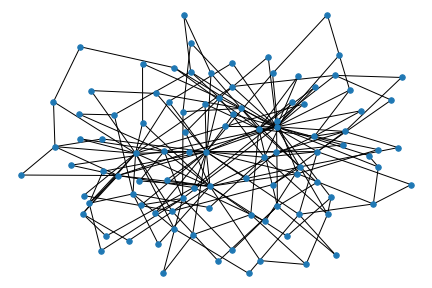
\includegraphics[width=0.9\linewidth]{figures/barabasi}
   \caption{}
   \label{fig:Ng1} 
\end{subfigure}

\begin{subfigure}[b]{0.5\textwidth}
  \centering
   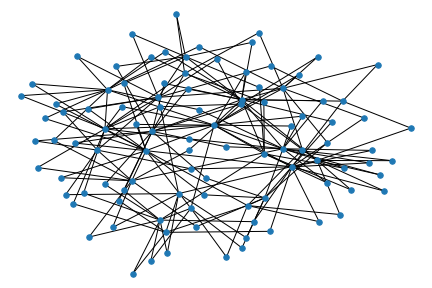
\includegraphics[width=0.9\linewidth]{figures/scafida}
   \caption{}
   \label{fig:Ng2}
\end{subfigure}

\caption{(a) Barabasi-Albert scale-free network w/ 100 nodes, w/o degree limitations
(b) Scafida topology w/ 100 nodes, and [10, 20, 10] switches of [4, 8, 16] ports}
\end{figure}

\subsection{Path Lengths}

We construct topologies using the Scafida algorithm, imposing uniform degree limitations to all switches. For each degree limit (port number) in \{8, 16, 24, 48, NL\}, NL standing for \textit{no limit}, we obtain the average shortest path length between all server pairs, i.e. the ratio of the sum of shortest path lengths to number of server pairs. Figure 2 shows a reproduction of figure 4a for various numbers of network nodes. The presented values are averaged over 50 topologies generated with the Scafida algorithm, and the value of m (degree of servers) is set to 2, which implies servers may be involved in the routing process. The original figure is presented along with the reproduced figure; it's apparent that they resemble each other closely, which suggests the Scafida re-implementation is successful. Observe that the average length of paths increases moderately with the number of nodes in the topology (for a given port number) due to the constrained degrees; in most cases, however, the increment is less than one full hop.

\begin{figure}[t]
\begin{subfigure}[b]{0.5\textwidth}
\centering
 \vspace{3pt}%
   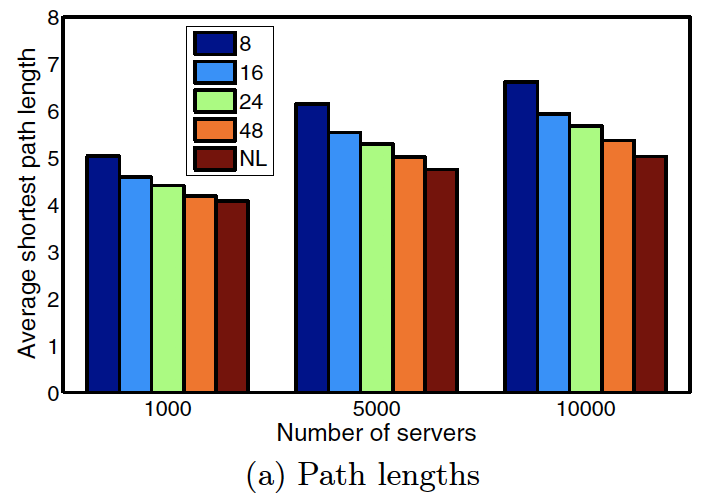
\includegraphics[width=0.95\linewidth]{figures/path_lengths_original}
   \caption{}
   \label{fig:Ng1} 
\end{subfigure}

\begin{subfigure}[b]{0.5\textwidth}
\centering
   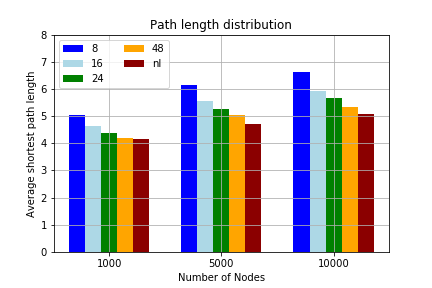
\includegraphics[width=0.95\linewidth]{figures/path_lengths}
   \caption{}
   \label{fig:Ng2}
\end{subfigure}

\caption{(a) Original Scafida paper average path length distribution over 50 simulations. (b) Reproduced figure of average path length distribution.}
\end{figure}

\subsection{Throughput}

The performance of communication-intensive applications relies heavily on the absence of bottlenecks in the topology. To quantify throughput, we explore the bisection bandwidth capabilities of the degree-constrained network in a realization with 5000 nodes. We assume that the links have uniform capacity, and that servers and switches alike have arbitrary throughput capability, i.e. do not constraint data flow. Since the network is too large for solving the minimum weight partition problem exactly, we instead use sampling. Specifically, we randomly partition the servers and switches in half, 200 times in total, after which the edge cut between the two sides of the network is computed. We then plot  the cumulative distribution function of bisection bandwidths, i.e.  edge cuts, in order to reproduce figure 4b of the original paper. Figure 3 presents the reproduced CDF function. The (amount of) degree limitation does not seem to affect the bisection bandwidth of the explored topologies, with all CDFs, including the one for the true scale-free network without degree limitations, roughly overlapping with each other.

\begin{figure}[t]
\begin{subfigure}[b]{0.5\textwidth}
\centering
   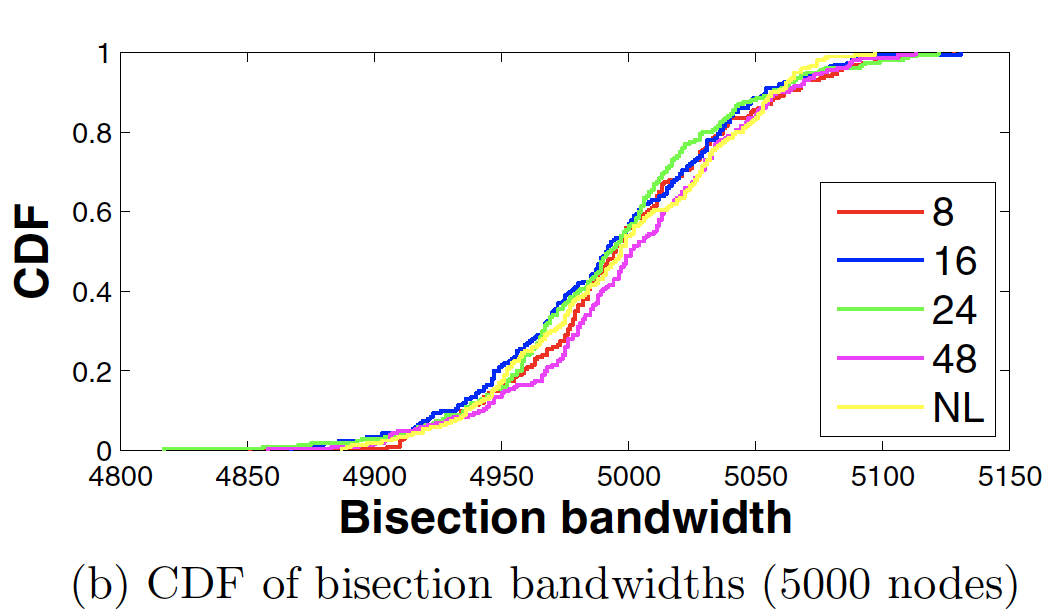
\includegraphics[width=0.95\linewidth]{figures/bisections_original}
   \caption{}
   \label{fig:Ng1} 
\end{subfigure}

\begin{subfigure}[b]{0.5\textwidth}
\centering
   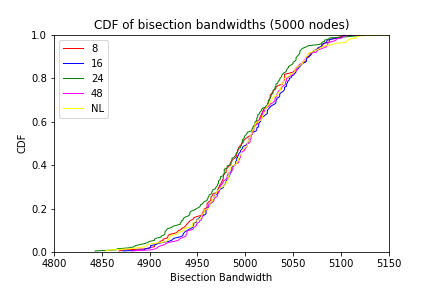
\includegraphics[width=0.95\linewidth]{figures/bisections}
   \caption{}
   \label{fig:Ng2}
\end{subfigure}

\caption{(a) Original paper CDF of bisection bandwidths on 5000-node topology over 200 random partitions of servers. (b) Reproduced CDF of bisection bandwidths.}
\end{figure}

\begin{figure}[t]

\begin{subfigure}[b]{0.5\textwidth}
\centering
   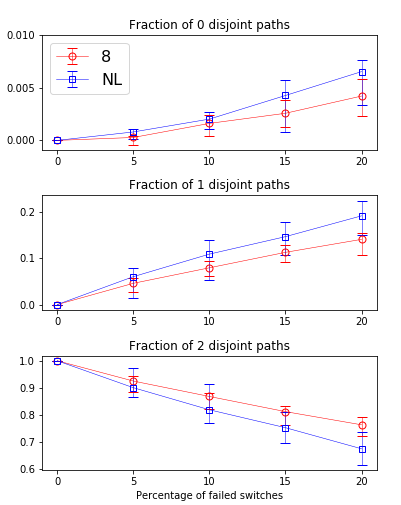
\includegraphics[width=0.95\linewidth]{figures/error}
   \caption{}
\end{subfigure}
\caption{(a) Original failure tolerance figure, showing percentage of server pairs connected by zero, one, and two disjoint paths, after a percentage of switches fail. (b) Reproduced error tolerance figure. }
\end{figure}

\subsection{Failure Tolerance}

Finally, we explore the tolerance to failure of the Scafida topology, and quantify the impact of constraining degree on the resilience of the architecture, using the same extreme cases as the original paper; namely, an unconstrained (true) scale-free network, as well as a Scafida topology with a degree limit of 8. In increments of five percent, from 0 and up to 20, we randomly remove switches and their adjacent edges from the network to mimic random switch failure in the datacenter. We then sample 4000 server pairs, selected uniformly at random, and compute the number of disjoint paths between them; since servers have a degree of 2, the maximum number of disjoint paths is also 2. Figure 4 plots a reproduction of the error tolerance experiments presented in the original paper's figure 5. The adjacent plots show the percentage of server pairs, connected by zero, one, and two \textit{disjoint} paths, respectively, for various fractions of randomly failed switches.

\section{Discussion \& Limitations}
First, let's consider the similarities, or lack thereof, of Scafida-generated topologies with other state-of-the-art network architectures. Figure 2 shows the average shortest path length in topologies with different network sizes, averaged over 50 simulations. Irrespective of the number of nodes in the network, constraining the degree increases average path lengths slightly, but usually less that 0.5 hops. As expected, for a given size, lower degree limitations result to slight increases in average path length. Although these measurements suggest that Scafida topologies result in shorter paths than other architectures, e.g. fat-trees, and shorter paths generally result to lower communication latency, it's not clear how much difference a one-hop increase in average path length makes in practice. We should therefore consider this statistic in conjunction with the trade-offs of a scale-free-like network, to be discussed shortly.

Depending on a datacenter's communication requirements, high throughput capability might be crucial for proper operation. Figure 3 shows that bisection bandwidth seems unaffected by degree limitations, which in turn suggests that a Scafida-generated network with varying numbers and types of equipment will likely display similar properties. Although, all else equal, the mean bisection bandwidth capabilities of Scafida topologies seem comparable to state-of-the-art architectures, they do not provide a strong argument for the use of the topology, since the complexities and haphazardness introduced by the iterative, scale-free approach may introduce other roadblocks that render it unfavorable.

In addition, resilience to failure is very important in the context of production data centers. Due to their probabilistic structure and random wiring, scale-free networks tolerate stochastic failures well. The original Scafida paper claims that degree constraints do not alter this favorable property, finding that even with 20\% of switches failing, more than 90\% of server pairs are still connected by two disjoint paths. This is the only result we were \textbf{unable} to reproduce with accuracy. Our numbers show that the Scafida topology is significantly \textit{less} resilient than suggested in the original paper; for instance, only around 70\% of server pairs are still connected by two disjoint paths in our reproduction. One likely explanation for this is the lack of specificity of the authors in describing the conditions of the experiment. Although they mention that 1000-node topologies were used, they do not specify the server-to-switch ratio, so it's up to anyone's guess what specific settings they used to generate their network. Throughout our experiments, when left unspecified, we tuned the settings to accommodate the maximum number of servers possible, given the equipment and degree limitations, and subject to the total number of nodes used, i.e. we maximized the number of servers. If the authors used a lower server-to-switch ratio, greater redundancy might have been created in the topology, which would explain the high failure tolerance measured in their experiments. It's worth noting, however, that  maximizing the server-to-switch ratio seems like the reasonable thing to do, in order to utilize the network's full capabilities. 

Although scale-free networks display favorable properties in theory, it's worth considering whether they are practical to implement and maintain in a production setting. Scafida's most significant advantage is the fine-grained control over network equipment that the algorithm allows for when creating a new topology. Unlike state-of-the-art architectures that use only few parameters, Scafida allows for maximal flexibility in terms of the type and amount of network equipment (servers and switches.) However, this introduces several problems. First, the algorithm allows no room for pre-planning of the topology; only after it terminates do nodes acquire meaningful roles, and as such there is no provision for incorporating a custom design even as a small part of the overall network. One possible solution to this might be to modify the initial steps of the algorithm and begin iteration on a pre-existing network "core", instead of an empty graph. The designer could explicitly decide which initial nodes other nodes can be attached to, and allow the Scafida algorithm to build a scale-free topology \textit{around} the core. Nevertheless, this doesn't account for the need to pre-plan server placement. Using the aforementioned approach would likely cause servers to be located in the \textit{middle} of the eventual architecture, which is where switches should instead be. We conclude that Scafida is not the best choice of architecture if fine-grained server placement is an important consideration in picking a data center topology.

Another significant barrier to practical materialization of Scafida networks, or more generally scale-free networks, is the complexity of the resulting topology. The haphazard nature of the cabling makes it significantly more labor-intensive to implement and maintain, renders both processes much more susceptible to human error, and might also increase material costs because of arbitrary cable lengths and unavoidable rewirings. Bundling, which was suggested as a potential solution to messiness of the wiring procedure in Jellyfish, doesn't seem promising, since it would only be practical for numbers of cables spanning the same area, and would make it harder to find and replace a given link; the alternative would be to provision for redundant cables in the bundles, which of course limits the amount of rewirings possible. Although incremental expansion is easy in theory, i.e. in terms of running the algorithm and obtaining an updated topology, it would likely be a nightmare to implement in a moderately-sized Scafida datacenter, and the difficulty would only scale with the size of the network.

\vspace{9pt}

\section{Conclusion}

In this work, we implement a version of the Scafida algorithm and evaluate numerous generated topologies. Although Scafida imposes degree constraints to nodes of a Barabasi-Albert topology, the network largely sustains the preferable properties of scale-free networks. Nevertheless, depending on the design goals, the complexity of implementation and maintenance may outweigh the benefits of flexibility and iterative expansion offered by Scafida.

\section{Github}

Source code, Jupyter notebooks, original and reproduced figures are available at github.com/steliosrousoglou/244-final.

\section{References}

\begin{itemize}[leftmargin=0pt]
       \item[] [1] A.-L. Barabási and R. Albert. Emergence of Scaling in Random Networks. Science, 286(5439):509–512, 1999.
       \vspace{4pt}
       \item[] [2] C. Guo, G. Lu, D. Li, H. Wu, X. Zhang, Y. Shi, C. Tian, Y. Zhang, and S. Lu. Bcube: a high performance, server-centric network architecture for modular data centers. In SIGCOMM ’09, pages 63–74, 2009.
       \vspace{4pt}
  \item[] [3] Gyaramati, L. and Tuan Ahn Trihn. Scafida: A Scale-Free Network Inspired Date Center Architecture. In SIGCOMM '10, vol. 40.
  \vspace{4pt}
  \item[] [4] Singla, A., Hong, C.-Y., Popa, L., and Godfrey, P. B. Jellyfish: Networking Data Centers Randomly. In NSDI (2012), vol. 12.
    \end{itemize}

